\documentclass{scrartcl}
\usepackage[utf8]{inputenc}
\usepackage{hyperref}
\usepackage{url}
\usepackage{natbib}
\usepackage{graphicx}
\usepackage{listings}
\usepackage{float}

\renewcommand{\labelenumii}{\arabic{enumi}.\arabic{enumii}}
\renewcommand{\labelenumiii}{\arabic{enumi}.\arabic{enumii}.\arabic{enumiii}}
\renewcommand{\labelenumiv}{\arabic{enumi}.\arabic{enumii}.\arabic{enumiii}.\arabic{enumiv}}

\newcommand{\emailaddr}[1]{\href{mailto:#1}{\texttt{#1}}}

\title{\LARGE
    CityTwin
}

% Consider watching:
% https://www.youtube.com/watch?v=ihxSUsJB_14
% https://www.youtube.com/watch?v=XTFWaV55uDo

\author{
    Filippo Vissani \\ \emailaddr{filippo.vissani@studio.unibo.it}
    \and 
    Eddie Barzi \\ \emailaddr{eddie.barzi@studio.unibo.it}
}

\date{September 2023}

\begin{document}

\maketitle

\begin{abstract}
    %Up to $\sim$2000 characters briefly describing the project.

    Il progetto CityTwin si propone di realizzare la simulazione di un sistema di digital twin nel contesto della smart city. In particolare, si vuole realizzare un sistema che sia in grado di catturare e rappresentare in formato digitale il comportamento delle varie entità presenti all'interno della città. Questo può portare ad una serie di benefici, alcuni dei quali vengono elencati di seguito:

    \begin{itemize}
        \item Rilevazione di possibili problematiche con intervento tempestivo e automatizzato.
        \item Riduzione del consumo energetico.
        \item Rilevazione della qualità dell'aria e dell'acqua.
        \item Analisi dell'inquinamento acustico.
        \item Ottimizzazione della mobilità urbana.
    \end{itemize}

    La simulazione sarà composta da due tipologie di nodi: i nodi Mainstay, che rappresentano la struttura portante del sistema, e i nodi Resource, che rappresentano astrazioni di sensori, attuatori o entità più complesse.

    I nodi Mainstay si occupano di scambiare informazioni con i nodi Resource, rilevare eventuali malfunzionamenti e salvare in modo persistente le informazioni rilevate dai nodi Resource. I nodi Mainstay devono essere sempre sincronizzati tra loro, in modo da poter garantire la coerenza dei dati.

    I nodi Resource, invece, si occupano di rilevare informazioni e comunicarle ai nodi Mainstay nel caso in cui vengano considerati come sensori. Nel caso in cui i nodi Resource rappresentino attuatori, invece, si occupano di ricevere informazioni dai nodi Mainstay e agire di conseguenza.

    Per la memorizzazione delle dello stato dei nodi viene disposto un servizio apposito di persistenza dei dati. Tale servizio viene utilizzato sia dai nodi Mainstay che da altri clienti, come ad esempio il pannello di controllo.

    L'utente potrà visualizzare lo stato attuale del sistema, lo storico dei dati ed eventuali statistiche, nonché interagire con il sistema tramite GUI, ad esempio per intervenire dopo la rilevazione di un incendio.

\end{abstract}

\section{Analisi dei requisiti}
In questa sezione verranno delineati i vari requisiti del sistema in base alle diverse categorie di requisiti identificate. Nella fase di analisi dei requisiti, abbiamo preso il ruolo di stakeholder per comprendere appieno le esigenze degli utenti e guidare lo sviluppo del sistema. Questo approccio ci ha permesso di metterci nei panni degli utilizzatori finali e di definire con precisione le azioni chiave che gli utenti avrebbero svolto all'interno del sistema.

\subsection{Requisiti di Business}
I requisiti aziendali definiscono gli obiettivi di alto livello e la motivazione dietro lo sviluppo del software. Rispondono alla domanda "perché?" e definiscono l'importanza strategica del progetto:
\begin{enumerate}
    \item Obiettivi Strategici: Il progetto "CityTwin" mira a creare una piattaforma di simulazione e monitoraggio delle smart city per migliorare la gestione e l'ottimizzazione delle risorse urbane.
    \item Aumento dell'Efficienza Urbana: Il sistema mira a migliorare l'efficienza operativa delle città intelligenti attraverso la rappresentazione digitale delle entità e delle interazioni all'interno della città.
\end{enumerate}

\subsection{Requisiti Utente}
I requisiti utente si concentrano sull'esperienza dell'utente finale e sulla modalità di interazione con il sistema.
Gli scenari d'uso hanno permesso di definire le azioni principali che gli utenti avrebbero potuto compiere all'interno dell'applicazione.
Per rappresentare in modo efficace questi scenari e facilitare la comunicazione visiva di quello che il sistema offre all'utente, è stato definito un diagramma dei casi d'uso, mostrato in Figura \ref{fig:use-cases-diagram}. Questo diagramma ha contribuito a visualizzare in modo chiaro ed esauriente le attività degli utenti e le interazioni con il sistema.

\begin{enumerate}
    \item L'utente deve avere a disposizione una GUI (Control Panel) con le seguenti funzionalità:
          \begin{enumerate}
              \item Deve mostrare lo stato attuale dei nodi Mainstay e Resource del sistema.
              \item Deve mostrare la posizione delle risorse nella città, indicandone il nome e lo stato (online/offline).
              \item Deve mostrare un grafico che rappresenti il numero di nodi Mainstay e Resource online nel tempo, sulla base dei dati rilevati
                    dal servizio di persistenza.
          \end{enumerate}
    \item L'utente deve avere a disposizione una GUI (River Monitor) con le seguenti funzionalità:
          \begin{enumerate}
              \item Deve mostrare lo stato attuale del River Monitor (Safe, Warned, Evacuating).
              \item Deve mostrare i sensori monitorati con il relativo livello dell'acqua.
              \item Deve mostrare il valore di soglia dell'acqua sopra la quale il River Monitor passa allo stato di "Warned".
              \item Deve mettere a disposizione un pulsante per passare allo stato di "Evacuating" e un pulsante per tornare allo stato di "Safe".
          \end{enumerate}
    \item L'utente deve avere la possibilità di aggiungere o rimuovere nuovi nodi Resource in tempo reale, senza che questo comprometta il funzionamento del sistema. Questa flessibilità consente di adattare il sistema alle mutevoli esigenze delle smart cities.
\end{enumerate}
\begin{figure}[H]
    \centering
    \caption{Diagramma dei casi d'uso.}
    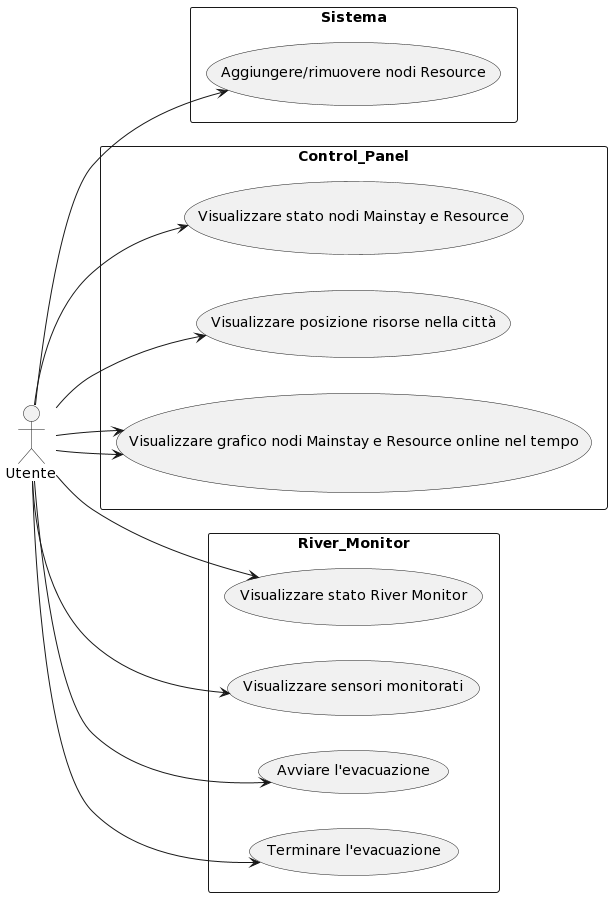
\includegraphics[width=0.8\textwidth]{../assets/images/use-cases-diagram.png}
    \label{fig:use-cases-diagram}
\end{figure}


\subsection{Requisiti Funzionali}
I requisiti funzionali delineano le funzioni specifiche del sistema, cioè cosa il sistema deve fare:
\begin{enumerate}
    \item I nodi Mainstay sono la struttura portante dell'intero sistema:
          \begin{enumerate}
              \item Ricevono informazioni dai nodi Resource che modellano sensori.
              \item Comunicano informazioni ai nodi Resource che modellano attuatori.
              \item Rilevano i malfunzionamenti dei nodi Resource.
              \item Rilevano i malfunzionamenti degli altri nodi Mainstay.
              \item Si occupano di salvare le informazioni contattando il servizio di persistenza.
              \item Non devono conoscere a prescindere le tipologie dei nodi Resource.
              \item Devono disporre di una struttura dati distribuita che permetta di memorizzare le informazioni rilevanti:
                    \begin{enumerate}
                        \item La struttura dati deve essere sincronizzata tra i nodi Mainstay.
                        \item La struttura dati deve mantenere la consistenza dei dati nel tempo.
                    \end{enumerate}
          \end{enumerate}
    \item I nodi Resource:
          \begin{enumerate}
              \item Rappresentano astrazioni di:
                    \begin{enumerate}
                        \item Sensori.
                        \item Attuatori.
                        \item Entità più complesse, come stazioni di controllo, che possono anche impiegare interfacce grafiche.
                    \end{enumerate}
              \item Fanno riferimento ad uno dei nodi Mainstay per ottenere o comunicare informazioni.
              \item Possono essere aggiunti o rimossi in tempo reale.
          \end{enumerate}
    \item Deve essere presente un servizio di persistenza dei dati che permetta di salvare in modo persistente:
          \begin{enumerate}
              \item Lo stato dei nodi Mainstay.
              \item Lo stato dei nodi Resource.
          \end{enumerate}
    \item Il malfunzionamento di un nodo non deve compromettere il funzionamento del sistema.
    \item Deve poter essere possibile introdurre nuovi moduli senza dover modificare i componenti esistenti.
    \item Vengono previsti i seguenti moduli per i nodi Resource:
          \begin{enumerate}
              \item Sensore per la rilevazione di piogge acide. Il sensore deve essere in grado di rilevare il valore di pH dell'acqua piovana, compreso tra 0 e 14.
              \item Sensore per l'analisi della qualità dell'aria. Il sensore deve essere in grado di rilevare i seguenti parametri chiave:
                    \begin{enumerate}
                        \item \label{itm:pm10} Concentrazione di PM10 (Particolato inferiore ai 10 micrometri).
                        \item \label{itm:pm25} Concentrazione di PM2,5 (Particolato inferiore ai 2,5 micrometri. Si noti che è un sottoinsieme del PM10).
                        \item \label{itm:NOx} Concentrazione di NOx (Ossidi di azoto).
                    \end{enumerate}
                    Si deve inoltre considerare che si andrà a utilizzare un sensore economico prefabbricato a basso consumo energetico, in grado di comunicare i dati rilevati tramite un protocollo di rete.
              \item Sensore per la rilevazione dell'inquinamento acustico, con le seguenti caratteristiche:
                    \begin{enumerate}
                        \item \label{itm:dB} Le letture devono variare in un intervallo di valori rappresentativi di un ambiente urbano, da 40 a 100 decibel (dB).
                        \item \label{itm:dBDescription} Oltre al valore in decibel, il sensore deve fornire una descrizione corrispondente al livello di rumore.
                    \end{enumerate}
              \item Modulo per la rilevazione del livello dell'acqua di un fiume e possibilità di intervento:
                    \begin{enumerate}
                        \item Sensore per la rilevazione degli allagamenti: il sensore deve periodicamente misurare il livello dell'acqua e comunicare il valore rilevato al nodo Mainstay.
                        \item Pannello di controllo per l'intervento in caso di allagamento, con le seguenti caratteristiche:
                              \begin{enumerate}
                                  \item Soglia di allagamento configurabile.
                                  \item Possibilità di controllare più sensori.
                                  \item Possibilità di assumere tre stati:
                                        \begin{itemize}
                                            \item Safe quando non c'è pericolo.
                                            \item Warned quando il livello dell'acqua supera la soglia di allagamento.
                                            \item Evacuating quando il livello dell'acqua supera la soglia di allagamento e l'utente ha premuto il pulsante di evacuazione.
                                        \end{itemize}
                                  \item Mostrare lo stato attuale del River Monitor.
                                  \item Passaggio in automatico allo stato Warned quando il valore della maggioranza dei sensori supera la soglia di allagamento.
                                  \item Possibilità di intervenire passando in stato Evacuating quando il sistema è Warned.
                                  \item Possibilità di intervenire tornando in stato Safe quando il sistema è Evacuating.
                              \end{enumerate}
                    \end{enumerate}
          \end{enumerate}
\end{enumerate}

\subsection{Requisiti Non Funzionali}
I requisiti non funzionali definiscono attributi di qualità, vincoli e proprietà generali del sistema:
\begin{enumerate}
    \item Affidabilità: L'affidabilità e la resilienza sono due aspetti cruciali del sistema "CityTwin". In caso di guasti hardware o malfunzionamenti dei nodi, il sistema deve essere in grado di mantenere la continuità delle operazioni fondamentali. A tale scopo, è prevista l'implementazione di un meccanismo di ridondanza, in cui i dati sono presenti in più istanze di nodi Mainstay.
    \item Performance: Il sistema deve rispondere tempestivamente alle richieste dell'utente (in media entro 1 secondo) e gestire grandi quantità di dati in tempo reale (almeno 30 risorse).
    \item Modularità: Il sistema deve essere realizzato in moduli separati, in modo da poter essere facilmente estendibile.
\end{enumerate}

\subsection{Requisiti di Implementazione}
I requisiti di implementazione riguardano gli aspetti tecnologici e metodologici dell'implementazione del sistema:
\begin{enumerate}
    \item Linguaggio di Programmazione: Il sistema deve essere realizzato utilizzando il linguaggio Scala 3.
    \item Architettura Basata su Attori: L'implementazione deve seguire il paradigma ad attori utilizzando il framework Akka per gestire l'interazione tra i nodi.
    \item Tecnologie di Persistenza: Il modulo di persistenza dei dati deve essere implementato utilizzando MongoDB per garantire la memorizzazione affidabile dei dati rilevati.
    \item Documentazione del Codice: Il codice deve essere adeguatamente documentato per consentire una comprensione chiara e agevolare la manutenzione futura.
\end{enumerate}

\section{Progettazione}

\subsection{Architettura del Sistema}

L'architettura del sistema, presentata in Figura \ref{fig:core-component-diagram}, è organizzata intorno a componenti interconnessi che consentono il monitoraggio e la gestione delle entità presenti all'interno della città. Ogni componente svolge ruoli specifici all'interno del sistema e interagisce attraverso interfacce ben definite.

\begin{figure}[H]
    \caption{Diagramma dei componenti del sistema e delle loro dipendenze.}
    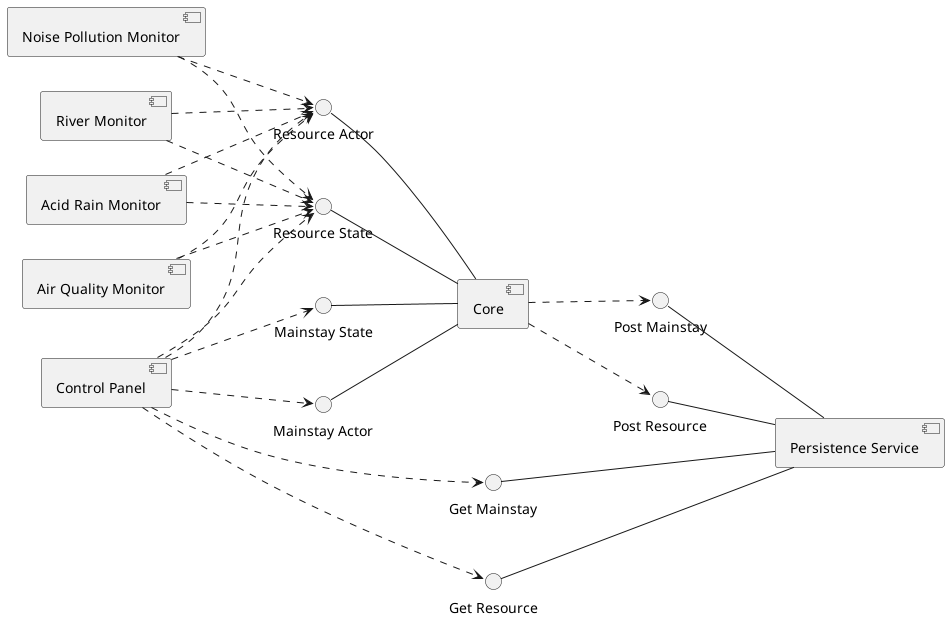
\includegraphics[width=\textwidth]{../assets/images/core-component-diagram.png}
    \label{fig:core-component-diagram}
\end{figure}

In Figura \ref{fig:nodes-component-diagram} viene presentata l'architettura dei componenti in esecuzione e dei protocolli di rete utilizzati. Il sistema è costituito da un insieme di nodi \textit{Mainstay} e \textit{Resource} che comunicano tra loro attraverso il protocollo \textit{Akka}. Inoltre, i nodi \textit{Mainstay} comunicano con il servizio di persistenza attraverso il protocollo \textit{HTTP}.
I nodi che comunicano utilizzando il protocollo \textit{Akka} sono \textit{Actor System} organizzati in un cluster, in modo da poter garantire la scalabilità del sistema.

\begin{figure}[H]
    \caption{Diagramma dei componenti in esecuzione e dei protocolli di rete utilizzati.}
    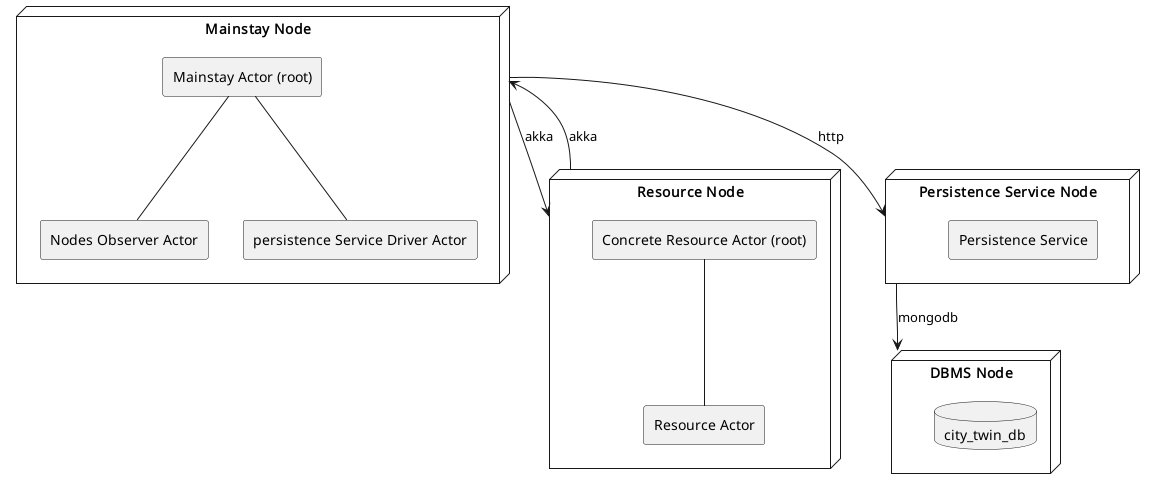
\includegraphics[width=\textwidth]{../assets/images/nodes-component-diagram.png}
    \label{fig:nodes-component-diagram}
\end{figure}

\subsubsection{Core}
Il componente centrale del sistema è il \textit{Core}, responsabile della gestione dell'elaborazione dati, del coordinamento delle attività e della comunicazione tra gli altri componenti. Il Core funge da mediatore tra le varie risorse presenti all'interno della città, ricevendo dati dai sensori e inviandoli al servizio di persistenza.

L'architettura del modulo \textit{Core} (Figura \ref{fig:core-class-diagram}) è costituita da diversi attori, ognuno dei quali svolge un ruolo specifico nel processo di acquisizione, gestione e comunicazione dei dati relativi alle risorse.

\textit{Resource Actor} è responsabile della gestione della risorsa, indipendentemente dal fatto che essa sia un sensore o un attuatore. Comunica con il \textit{Mainstay Actor} per ottenere o mandare lo stato delle risorse. È in grado di ricevere comandi e cambiamenti relativi alle risorse.

Il \textit{Mainstay Actor} si occupa di tenere in piedi l'intero sistema distribuito. Esso scambia lo stato delle risorse con il \textit{Resource Actor} e comunica con il \textit{Persistence Service Driver Actor} per salvare i dati nel servizio di persistenza. Inoltre, il \textit{Mainstay Actor} è responsabile della sincronizzazione dei nodi \textit{Mainstay}.

Il \textit{Nodes Observer Actor} monitora gli stati dei nodi all'interno del sistema e aggiorna il \textit{Mainstay Actor} sulla base del cambiamento di stato dei nodi.

L'attore \textit{Persistence Service Driver} è responsabile della gestione delle operazioni di persistenza dei dati. Comunica con il \textit{Mainstay Actor} per pubblicare nuovi dati al servizio di persistenza.

L'architettura prevede interazioni chiare e ben definite tra gli attori attraverso l'utilizzo di comandi specifici.

Il \textit{Resource Actor} comunica con il \textit{Mainstay Actor} utilizzando comandi come \textit{AskResourcesState}, \textit{AskAllResourcesState} e \textit{UpdateResources}. Queste interazioni consentono al \textit{Resource Actor} di ottenere informazioni sullo stato delle risorse e di aggiornare lo stato stesso.

Il \textit{Mainstay Actor} comunica con il \textit{Persistence Service Driver Actor} utilizzando comandi come \textit{PostMainstay} e \textit{PostResource}. Queste interazioni consentono al \textit{Mainstay Actor} di inviare nuovi dati al servizio di persistenza.

\begin{figure}[H]
    \caption{Diagramma delle classi del modulo \textit{Core}.}
    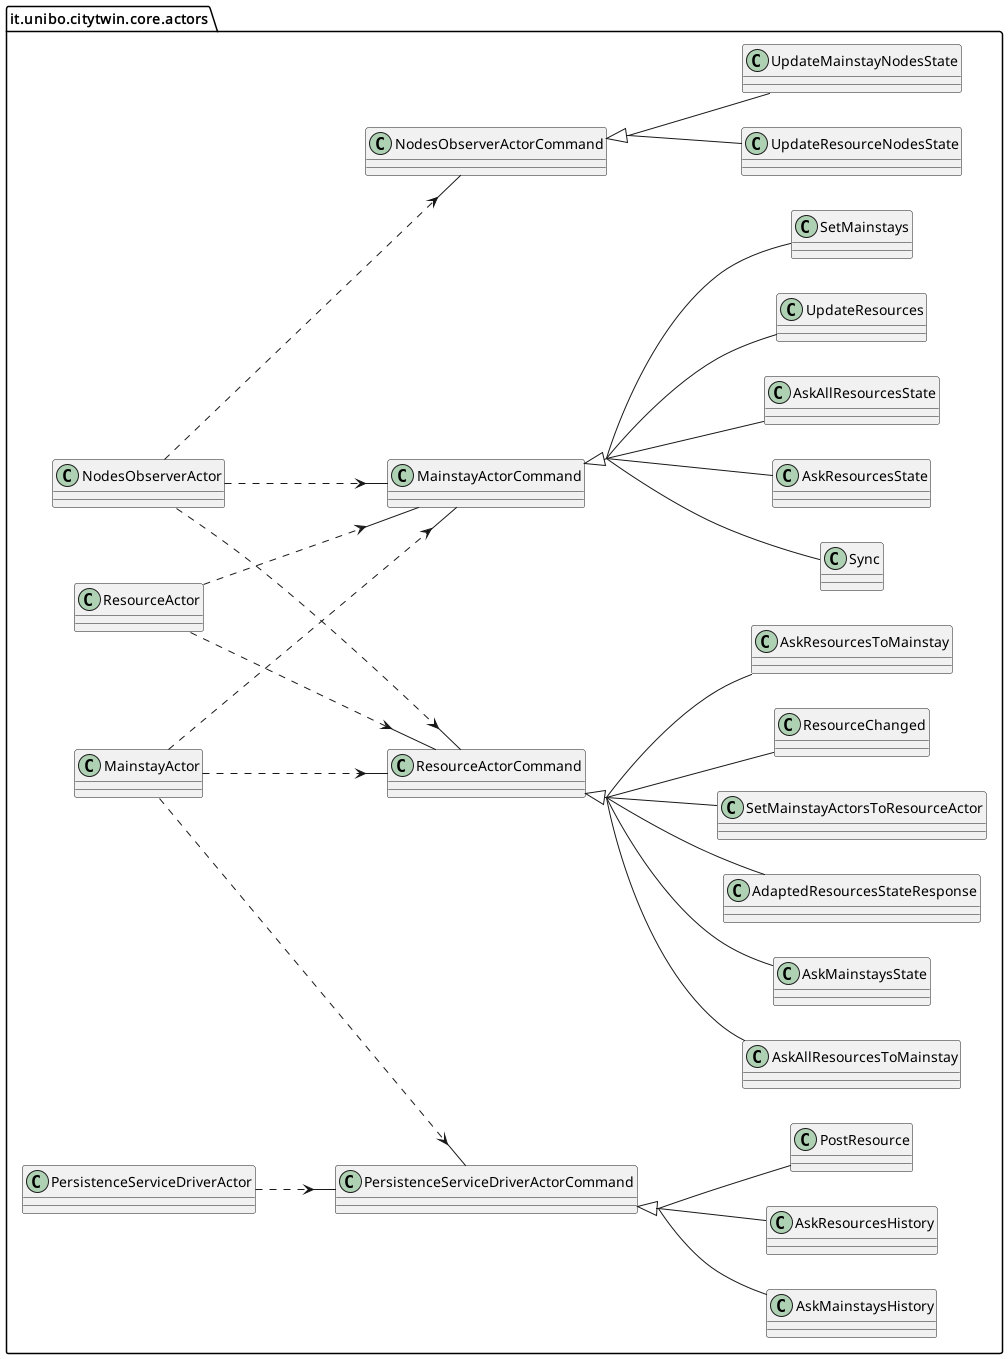
\includegraphics[width=\textwidth]{../assets/images/core-class-diagram.png}
    \label{fig:core-class-diagram}
\end{figure}

\subsubsection{Componenti Monitor}
I diversi monitor ambientali, come l'\textit{Acid Rain Monitor}, l'\textit{Air Quality Monitor}, il \textit{Noise Pollution Monitor} e il \textit{River Monitor}, costituiscono le fonti primarie di dati. Ciascun monitor raccoglie misurazioni specifiche e invia queste informazioni al \textit{Core} tramite l'interfaccia \textit{Resource}. Questa comunicazione consente al \textit{Core} di elaborare i dati e fornire una visione completa delle condizioni ambientali.

\subsubsection{Control Panel}
Il \textit{Control Panel} è l'interfaccia utente principale attraverso cui gli utenti interagiscono con il sistema. Comunica con il \textit{Core} per ottenere dati sullo stato ambientale e sul sistema nel suo complesso. Inoltre, il pannello di controllo richiede al servizio di persistenza lo storico dei dati in modo da poterli elaborare per ottenere delle statistiche.

\subsubsection{Persistence Service}
Il \textit{Persistence Service} gestisce la persistenza dei dati nel sistema. Comunica con il \textit{Core} attraverso le interfacce \textit{Post Resource} e \textit{Post Mainstay} per ricevere e salvare i dati relativi alle risorse. Analogamente, le interfacce \textit{Get Mainstay} e \textit{Get Resource }consentono di richiedere i dati al servizio di persistenza.

\subsection{Behaviour}

TODO

\subsection{Interazioni dei Componenti}

Il comportamento generale del sistema viene definito sulla base di una serie di interazioni tra i componenti. In particolare, le interazioni possono essere raggruppate per definire un determinato aspetto di tale comportamento.

\subsubsection{Aggiornamento Sullo Stato dei Nodi}

Lo scambio di messaggi tra \textit{Nodes Observer Actor} e \textit{Mainstay Actor} (Figura \ref{fig:core-nodes-state-sequence-diagram}) è volto a mantenere aggiornato quest'ultimo sullo stato generale dei nodi del sistema. Nel momento in cui il \textit{Mainstay Actor} riceve un aggiornamento sui nodi, esso aggiorna il proprio stato e lo comunica al \textit{Persistence Service Driver Actor}, che si occupa di rendere persistenti i dati tramite il servizio di persistenza.

\begin{figure}[H]
    \caption{Diagramma di sequenza per l'aggiornamento sullo stato dei nodi del sistema.}
    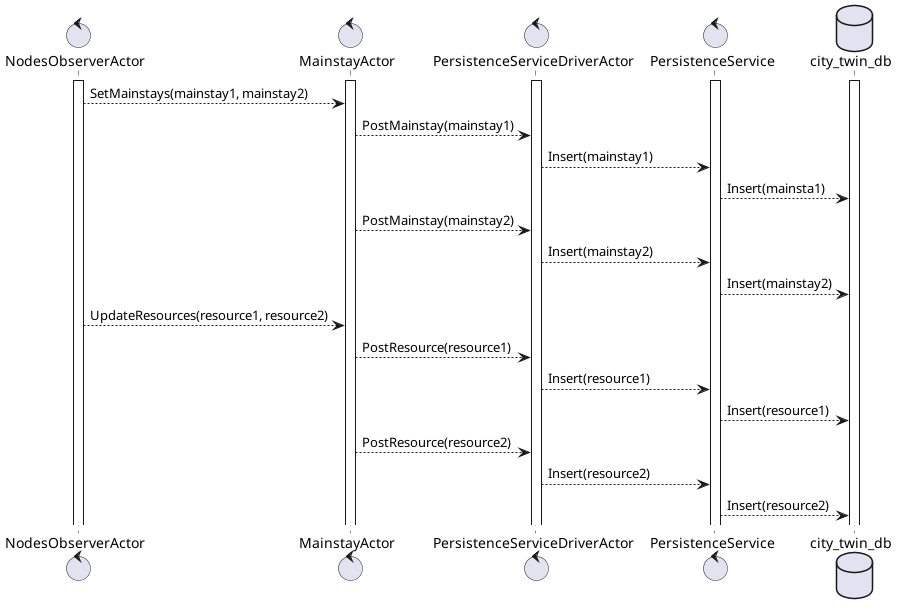
\includegraphics[width=\textwidth]{../assets/images/core-nodes-state-sequence-diagram.png}
    \label{fig:core-nodes-state-sequence-diagram}
\end{figure}

\subsubsection{Aggiornamento Sullo Stato delle Risorse}

Lo scambio di messaggi tra \textit{Resource Actor} e \textit{Mainstay Actor} (Figura \ref{fig:core-resource-state-exchange-sequence-diagram}) è utile a:
\begin{itemize}
    \item Ottenere lo stato delle altre risorse e comunicare il proprio nel caso un cui il nodo \textit{Resource} modella un attuatore.
    \item Comunicare lo stato della risorsa nel caso un cui il nodo \textit{Resource} modella un sensore.
\end{itemize}

In ogni caso, quando il \textit{Mainstay Actor} riceve un aggiornamento, lo comunica al servizio di persistenza tramite il \textit{Persistence Service Driver Actor}.

\begin{figure}[H]
    \caption{Diagramma di sequenza per lo scambio dello stato delle risorse.}
    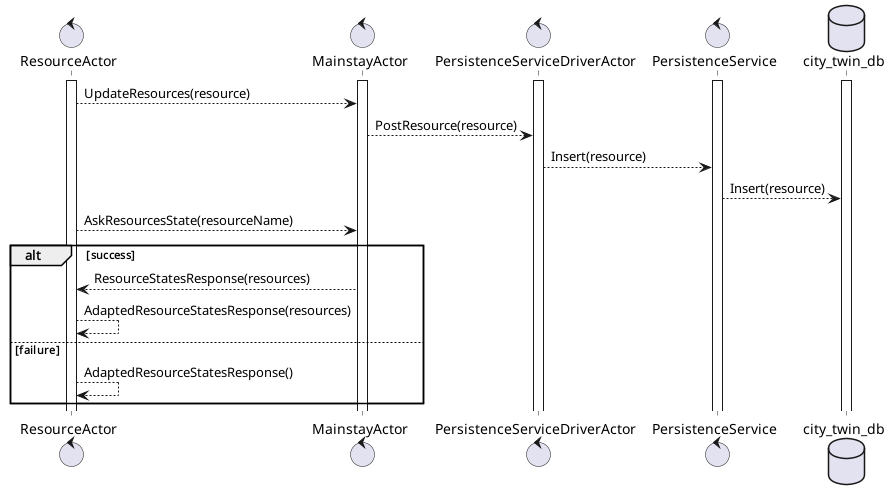
\includegraphics[width=\textwidth]{../assets/images/core-resource-state-exchange-sequence-diagram.png}
    \label{fig:core-resource-state-exchange-sequence-diagram}
\end{figure}

\subsubsection{Sincronizzazione dei Nodi Mainstay}

Come detto precedentemente, i nodi \textit{Mainstay} sono i pilastri portanti dell'intero sistema e si occupano della gestione dei dati riguardanti le risorse e i nodi. I nodi \textit{Mainstay} devono essere sempre sincronizzati tra loro, in modo da poter garantire la coerenza dei dati. Per questo motivo, i nodi \textit{Mainstay} si sincronizzano ogni volta che una risorsa manda il suo stato ad uno di questi. In Figura \ref{fig:core-mainstays-sync-sequence-diagram} viene presentato il diagramma di sequenza per la sincronizzazione dei nodi \textit{Mainstay}.

\begin{figure}[H]
    \caption{Diagramma di sequenza per la sincronizzazione dei nodi Mainstay.}
    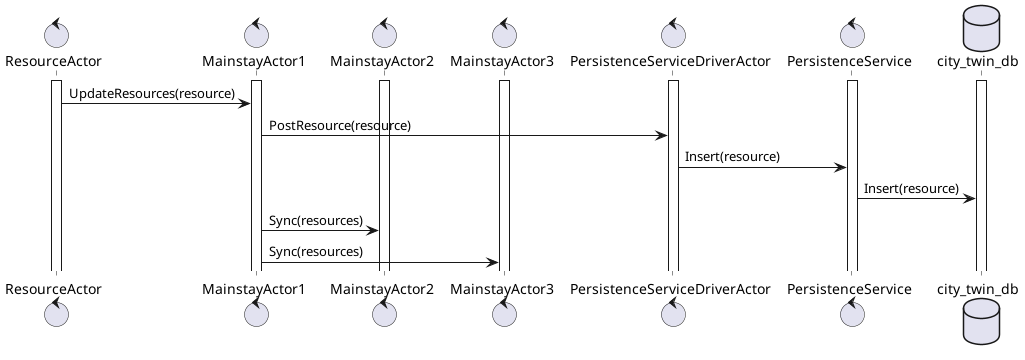
\includegraphics[width=\textwidth]{../assets/images/core-mainstays-sync-sequence-diagram.png}
    \label{fig:core-mainstays-sync-sequence-diagram}
\end{figure}

\subsubsection{Aggiornamento del Pannello di Controllo}

Il comportamento del \textit{Control Panel} (Figura \ref{fig:control-panel-sequence-diagram}) viene modellato come un caso particolare di risorsa che comunica con il \textit{Mainstay Actor} per ottenere lo stato delle risorse e dei nodi. Inoltre, il \textit{Control Panel} comunica con il servizio di persistenza per ottenere lo storico dei dati e calcolare le statistiche.

\begin{figure}[H]
    \caption{Diagramma di sequenza per l'aggiornamento del pannello di controllo.}
    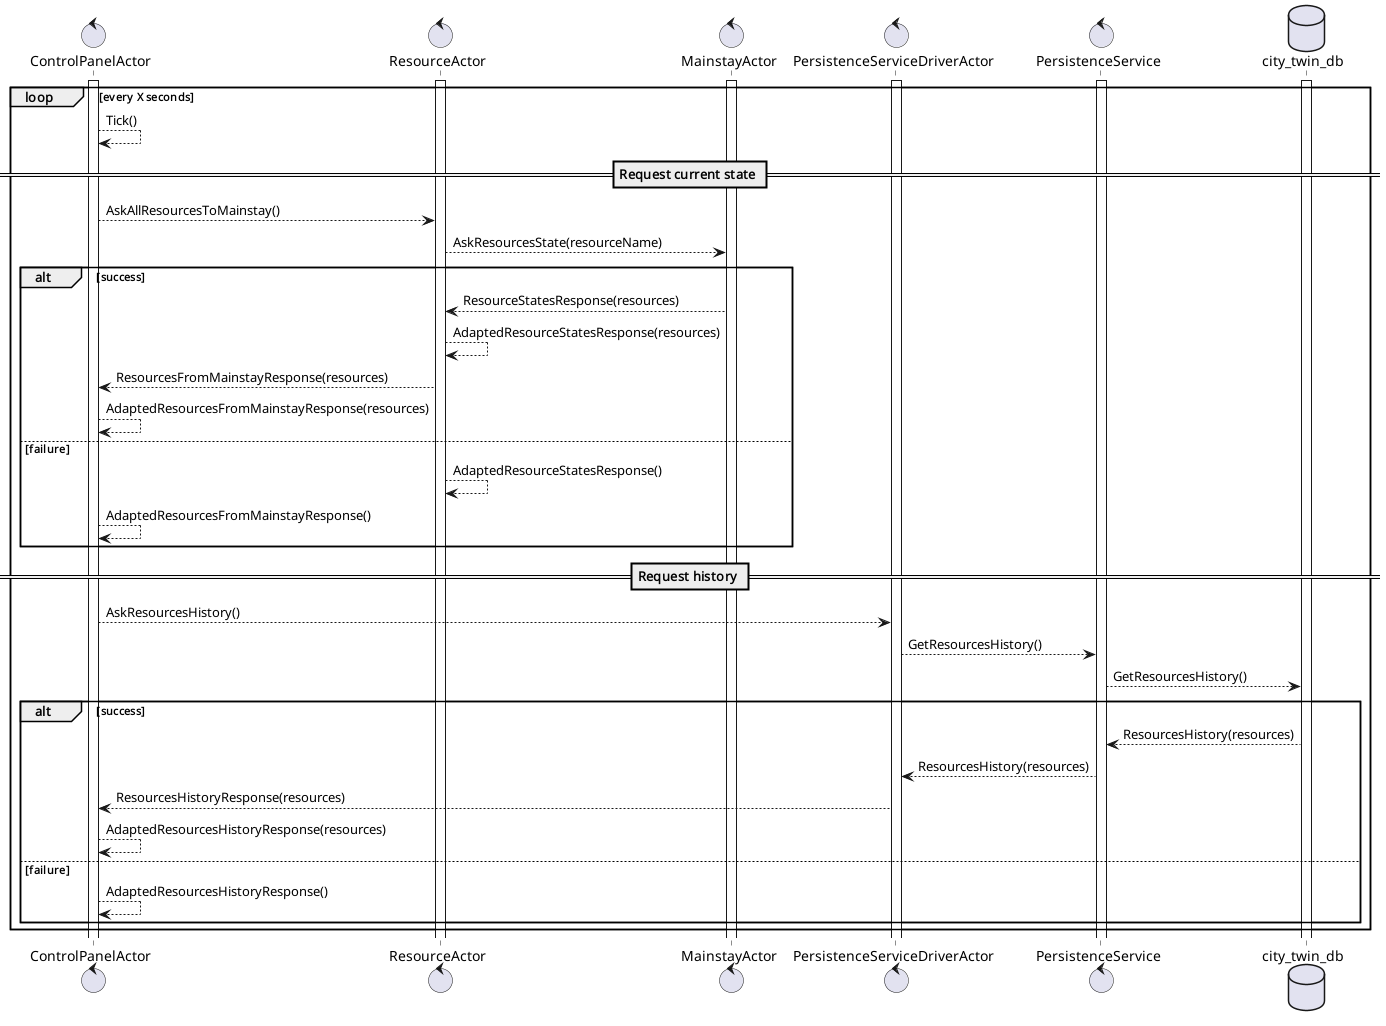
\includegraphics[width=\textwidth]{../assets/images/control-panel-sequence-diagram.png}
    \label{fig:control-panel-sequence-diagram}
\end{figure}

\section{Implementation Details}

Just report interesting / non-trivial / non-obvious implementation details.

This section is expected to be short in case some documentation (e.g. Javadoc or Swagger Spec) has been produced for the software artefacts.
%
This this case, the produced documentation should be referenced here.

\section{Self-assessment / Validation}

Choose a criterion for the evaluation of the produced software and \textbf{its compliance to the requirements above}.

Pseudo-formal or formal criteria are preferred.

In case of a test-driven development, describe tests here and possibly report the amount of passing tests, the total amount of tests and, possibly, the test coverage.

\section{Istruzioni per il Deploy}

%Explain here how to install and launch the produced software artefacts.
%
%Assume the softaware must be installed on a totally virgin environment.
%
%So, report \textbf{any} configuration step.

%Gradle and Docker may be useful here to ensure the deployment and launch processes to be easy.
\subsection{Requisiti in comune}
\begin{itemize}
    \item Scala 3.3.0
    \item Java openjdk 17.0.7
    \item SBT 1.x
    \item Docker
    \item Docker Compose
\end{itemize}

\subsection{Requisiti specifici per piattaforma}
\subsubsection{Linux}
\begin{itemize}
    \item unzip
\end{itemize}

\subsubsection{Windows}
\begin{itemize}
    \item Powershell
    \item tar
\end{itemize}

\section{Avvio del sistema}

%Show how to use the produced software artefacts.

%Ideally, there should be at least one example for each scenario proposed above.

Prima di tutto, avviare il servizio di persistenza:

\begin{lstlisting}[language=bash]
    docker compose build
    docker compose up
\end{lstlisting}
Quindi avviare il resto del sistema in un altro terminale:

Su Linux (bash):

\begin{lstlisting}[language=bash]
    ./scripts/startup.sh
\end{lstlisting}

Su Windows (Powershell):

\begin{lstlisting}[language=bash]
    ./scripts/startup.bat
\end{lstlisting}

\section{Conclusioni}

%Recap what you did
In conclusione possiamo evidenziare come il progetto abbia raggiunto gli obiettivi prefissati, ovvero la realizzazione di un sistema distribuito per il monitoraggio di una Smart City. Il sistema è stato sviluppato in maniera modulare, in modo da poter essere facilmente esteso e mantenuto. Inoltre, il sistema è stato progettato per essere scalabile e resiliente, in modo da poter essere utilizzato in un contesto reale.

\subsection{Sviluppi futuri}

%Recap what you did \emph{not}
Tra i vari miglioramenti a cui abbiamo pensato, i più significativi sono:
\begin{itemize}
    \item Utilizzo di una mappa geografica reale (simile a \textit{Google Maps}): Integrare una mappa geografica reale all'interno del sistema, consentendo di posizionare le risorse virtuali in base alle coordinate reali delle smart city. Questo migliorerebbe la precisione della modellazione e consentirebbe una rappresentazione più accurata dell'ambiente urbano.
    \item Sviluppo delle interfacce grafiche con applicazioni web in modo da renderle accessibili da dispositivi di vario genere (computer, smartphone, tablet, ecc.).;
    \item Possibilità per le risorse di tipo \textit{Act} di accedere allo storico dei dati rendendo trasparente il servizio di persistenza;
    \item Sostituzione dei sensori virtualizzati con sensori reali, in modo da poter effettuare un deployment su larga scala in un contesto reale.
    \item Implementazione di un sistema di autenticazione e autorizzazione per garantire la sicurezza del sistema.
    \item Implementazione di un sistema di notifiche per avvisare gli utenti in caso di eventi critici.
    \item Espansione delle funzionalità di analisi con l'ausilio di sistemi \textit{Big Data}: Introduzione di capacità di analisi avanzate per estrarre insight più profondi dai dati raccolti, ad esempio, analisi predittive per prevedere eventi futuri o rilevare anomalie in tempo reale.
    \item Implementazione di AI e Machine Learning: Integrazione di algoritmi di intelligenza artificiale e machine learning per l'automazione delle decisioni basate sui dati e per migliorare l'efficienza operativa delle smart city.
\end{itemize}

\subsection{What did we learned}

Racap what did you learned

\nocite{*} % Includes all references from the `references.bib` file
\bibliographystyle{plain}
\bibliography{references}

\end{document}
